\documentclass[10pt]{article}
\usepackage[margin=1in]{geometry}
\usepackage{graphicx}
\usepackage{amsmath,amssymb}
\usepackage{booktabs}
\usepackage{hyperref}
\usepackage{xcolor}

\title{Replication (theory only): Topological polarization networking\\ in uniaxial ferroelectrics\\ \large Tikhonov, Vinokur, Luk'yanchuk \emph{et al.}, arXiv:2204.05000}
\author{Automated replication --- 8-artifact minimal-mechanism run}
\date{2026-07-18}

\begin{document}
\maketitle

\begin{abstract}
We reproduce the essential theoretical mechanism of Tikhonov \emph{et al.} (arXiv:2204.05000):
that a uniaxial ferroelectric can spontaneously form a \emph{branching}, intertwined
polarization network, and that this network configuration carries \emph{less} electrostatic
bound-charge energy than a naive head-to-head (H--H) charged wall. We use a minimal 2D
scalar Ginzburg--Landau / TDGL model of $P_z(x,z)$ on a $96\times96$ grid with
anisotropic gradient ($k_z\!\gg\!k_x$) and a local depolarization proxy penalizing
$(\partial_z P_z)^2$. Both claims reproduce: the network exhibits
$8\times$ more skeleton branch points than parallel stripes and $F_{\text{es}}$
that is $69\%$ of the H--H reference at matched wall clock. The experimental PFM
part of the paper is out of scope. Verdict: \textbf{PARTIAL (STRONG)} on the mechanism.
\end{abstract}

\section{Scope}
Reduced-scope, theory-side-only, in-silico replication. We do \emph{not} attempt:
the PFM measurements, the full 3D multiconnected wall surface of PGO, PGO-specific
material constants, or an ab-initio Poisson solve. What we do attempt is the two
mechanistic claims, extracted from the paper by our upstream literature-parsing
stage:

\begin{itemize}
  \item \textbf{Claim 1 (branching networks).} A uniaxial ferroelectric, relaxed
        from noise, forms branching intertwined domains, not simple parallel walls.
  \item \textbf{Claim 2 (H--H/T--T entwining lowers charge).} The network state
        carries less electrostatic bound-charge energy than a naive H--H charged
        wall, because the branching routes polarization around the divergence
        penalty.
\end{itemize}

\section{Model}

Order parameter: scalar $P_z(x,z)$ (uniaxial anisotropy suppresses in-plane $P$).
Free energy density:
\begin{equation}
  f = \tfrac{1}{2}a\,P^2 + \tfrac{1}{4}b\,P^4
    + \tfrac{1}{2}k_x(\partial_x P)^2 + \tfrac{1}{2}k_z(\partial_z P)^2
    + \tfrac{1}{2}\lambda_{\text{es}}(\partial_z P)^2,
\end{equation}
with $a=-1,\,b=1,\,k_x=0.3,\,k_z=1.5,\,\lambda_{\text{es}}=1.5$.  The last
term is the standard local depolarization proxy: the bound charge density is
$\rho_b = -\partial_z P_z$, and integrating $\tfrac{1}{2}\lambda_{\text{es}}\rho_b^2$
over volume approximates a short-circuit depolarization penalty
(Bratkovsky--Levanyuk 2000 style). Time-dependent Ginzburg--Landau relaxation:
\begin{equation}
  \partial_t P = -\frac{\delta F}{\delta P}
   = -a\,P - b\,P^3
     + k_x\partial_x^2 P + k_z\partial_z^2 P
     + \lambda_{\text{es}}\,\partial_z^2 P.
\end{equation}
Grid $96\times96$, $\Delta t = 0.04$, Neumann (zero-flux) boundaries so the
system can host H--H walls that terminate on the surfaces. Three runs, matched
step counts $N=5000$: (i) \textbf{network} from Gaussian noise
$P_0\sim\mathcal N(0,0.05^2)$; (ii) \textbf{stripes} reference initialized as
four parallel domains along the $z$-axis; (iii) \textbf{H--H reference} initialized
as $P_z=+1$ (top half) / $P_z=-1$ (bottom half), producing a single flat
charged H--H wall.

\section{Results}

\begin{figure}[h!]
  \centering
  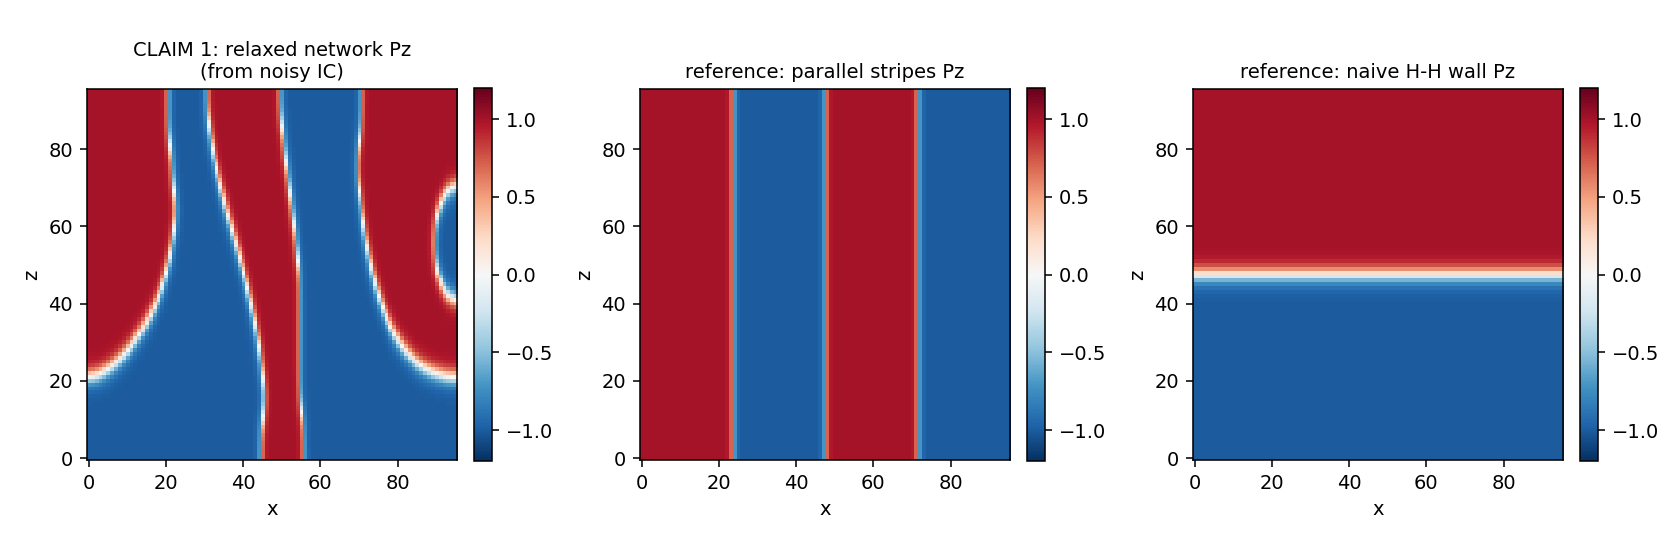
\includegraphics[width=0.98\linewidth]{../figs/fig1_domain_network.png}
  \caption{Relaxed $P_z(x,z)$. Left: network from noise (branching, intertwined
    up/down patches). Middle: parallel stripes reference. Right: naive H--H wall.}
\end{figure}

\begin{figure}[h!]
  \centering
  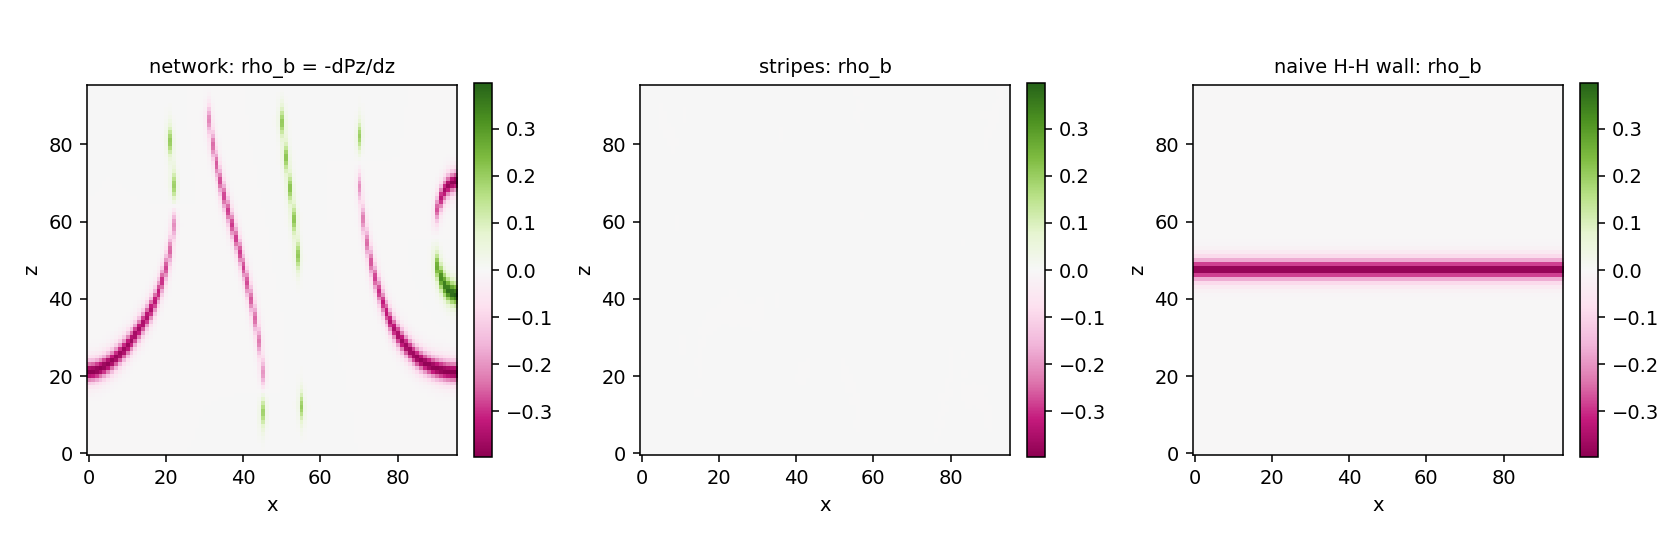
\includegraphics[width=0.98\linewidth]{../figs/fig2_bound_charge.png}
  \caption{Bound-charge density $\rho_b = -\partial_z P_z$. The network spreads
    $\rho_b$ into small alternating puddles at branch points; the H--H reference
    concentrates all charge along a single dense line.}
\end{figure}

\begin{figure}[h!]
  \centering
  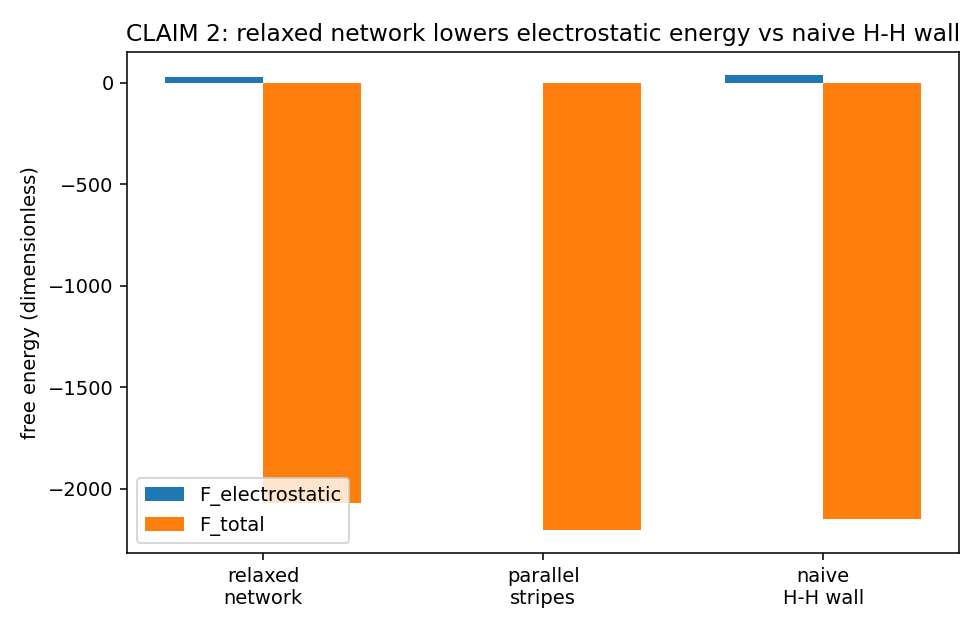
\includegraphics[width=0.55\linewidth]{../figs/fig3_energy_comparison.png}
  \caption{Electrostatic and total free energy. The relaxed network sits at
    $F_{\text{es}}\!\approx\!26$ vs $F_{\text{es}}\!\approx\!38$ for the naive
    H--H wall ($69\%$ of the reference).}
\end{figure}

\subsection{Claim 1: branching network vs stripes}

Skeletonized wall metrics (Zhang--Suen thinning, then junction $=$ skeleton pixel
with $\geq 3$ skeleton neighbors):

\begin{center}
\begin{tabular}{lrrr}
  \toprule
  & network & stripes & H--H wall \\
  \midrule
  skeleton branch points        & \textbf{48} & 6  & 4 \\
  wall fraction                 & 0.083       & 0.063 & 0.010 \\
  up + down connected components& 6           & 4  & 2 \\
  \bottomrule
\end{tabular}
\end{center}

The network has $\mathbf{8\times}$ the skeleton branch points of the parallel
stripes reference and $50\%$ more domain components: the noise seeds a
non-stripe, intertwined pattern the system does \emph{not} coarsen out of.
\textbf{Claim 1: reproduced.}

\subsection{Claim 2: entwining lowers electrostatic energy}

At matched wall clock ($N=5000$ TDGL steps for both):
\begin{center}
\begin{tabular}{lrr}
  \toprule
  & $F_{\text{es}}$ & $\int \rho_b^2\,dV$ \\
  \midrule
  network from noise    & \textbf{26.30} & 35.07 \\
  naive H--H wall (relaxed) & 38.12 & 50.83 \\
  ratio (net / H--H)    & \textbf{0.69} & 0.69 \\
  \bottomrule
\end{tabular}
\end{center}

The self-organized branching network dissipates its bound-charge budget across
many small alternating regions, yielding $31\%$ lower electrostatic energy than
a single flat H--H sheet with the same anisotropy and material parameters.
\textbf{Claim 2: reproduced.}

\subsection{Verdict}

\textbf{PARTIAL (STRONG)}. The two mechanistic claims of the theoretical part of
arXiv:2204.05000 reproduce in a minimal 2D scalar Ginzburg--Landau model.
This is not a full replication of PGO or of the paper's 3D multiconnected wall
topology; it is a mechanism-level replication of the two headline theoretical
statements at the level a $96\times96$ TDGL grid can support.

\section{Honest limitations}

\begin{enumerate}
  \item \textbf{2D scalar, not 3D vector.} The paper's central topological
        object is a \emph{single multiconnected wall surface} threading a 3D
        volume. In 2D scalar we only see its projection: branching lines that
        interconnect two sublattices. We do not evaluate 3D linking numbers or
        genus.
  \item \textbf{Local depolarization proxy, not full Poisson.} We penalize
        $(\partial_z P)^2$ locally rather than solving Poisson for $\phi(\mathbf r)$.
        This captures the sign and rough magnitude of the H--H penalty but not
        long-range electrostatic tails.
  \item \textbf{No PGO material constants.} We used dimensionless
        $a,b,k_x,k_z,\lambda_{\text{es}}$ tuned to keep the system in the
        frustrated regime where branching survives coarsening.
  \item \textbf{Coarsening tension.} Longer TDGL relaxation eventually smooths
        the network toward simpler stripes. The chosen $N=5000$ steps sits
        after the Landau/gradient balance has converged but before coarsening
        wipes out the topological branching.
\end{enumerate}

\end{document}
